\documentclass[10.5pt,a4paper]{letter}
\usepackage[top=0.75in, bottom=0.75in, left=0.75in, right=0.75in]{geometry}
\usepackage{graphicx}
\usepackage{natbib}

\begin{document}

\begin{letter}{}
\includegraphics[width=0.2\textwidth]{/Users/aileneettinger/Dropbox/Documents/Work/AA_heading.pdf}

\opening{Dear Dr. Lei:}
\par We propose a manuscript for \emph{Nature Plants} that addresses an urgent question in plant ecology: What are the implications
of the altered photoperiod that plants experience with climate change-induced shifts in their ranges and seasonal
activities? The two most-observed biological impacts of climate change are shifts in space (range shifts) and time (phenological shifts). Both alter experienced photoperiod, which could dramatically affect performance and fitness. However, the magnitude of effects from shifts in photoperiod with climate change are unknown or unquantified for most species. This manuscript would combine aspects of both a `Review' and a `Perspective,' and thus we believe would be appropriate in either format. We include below a proposed abstract and figures.

\par In the proposed manuscript we synthesize the large body of controlled environment experiments that test effects of temperature and photoperiod on spring phenology (\emph{1}). Our review differs from previous work  (\emph{e.g., 2,3}) by quantifying expected changes in experienced photoperiod due to shifts in space versus time (Fig. 1). It would be broadly relevant, as photoperiod acts as a cue for the spring emergence of diverse plant species, and altered photoperiod can affect plant development, growth, and fitness. Understanding these changes is critical for scientists studying basic ecology, with extensions to cellular and molecular biology research relating to photoperiod. The work also has relevance to how we forecast plant and ecosystem responses to climate change, since implications of climate change-induced shifts in photoperiod are largely unexplored, especially for early-season spring events, where---we argue---changes may be dramatic.

\par This piece would be timely and important because of its focus on the intersection of photoperiod and spring phenology (similar to \emph{4,5,6})---this is an area of growing interest given recent studies suggesting that photoperiod may underlie declining responses to warming (\emph{e.g., 7}). To date, the role of photoperiod has received far more detailed attention for end-of-season activities, such as growth cessation in the fall, than for spring activities. Though photoperiod cues dominate in the fall for many organisms, fall phenology responses to climate change have been muted. In contrast, spring phenology responds strongly to temperature and thus has advanced substantially with warming causing cascading, and generally unexplored, effects on photoperiod experienced at the start of spring. We demonstrate that incorporating photoperiod into forecasts is possible by leveraging existing experimental data: as an example, we show that growth chamber experiments on woody plant spring phenology often have data relevant for climate change impacts (e.g., Fig. 2). 

\par Our international team includes researchers well-versed in techniques of controlled climate experiments, having conducted such studies ourselves (e.g., \emph{8}), as well as scientists with expertise in meta-analytical approaches (e.g., \emph{9,10}). We expect our proposed `Review' or `Perspective' will inspire innovative research to
improve mechanistic understanding of photoperiod as a cue for diverse biological processes, as well as a deeper appreciation for the ways that experienced photoperiod may both affect and be affected by plant responses to climate change; we hope you will consider it for \emph{Nature Plants}.

\par Sincerely,\\

\includegraphics[scale=.3]{/Users/aileneettinger/Dropbox/Documents/Work/AileneEttingerSignature.png} \\
Ailene Ettinger
\begin{footnotesize}\\
Quantitative Ecologist, The Nature Conservancy- Washington Field Office\\
Visiting Fellow, Arnold Arboretum of Harvard University 
\end{footnotesize}

\newpage
\noindent {\bf Spatial and temporal shifts in photoperiod with climate change}\\
\\
\noindent \emph{Authors:} A.K. Ettinger, D.M. Buonaiuto, C.J. Chamberlain, I. Morales-Castilla \& E.M. Wolkovich
\\

Climate change causes both temporal (e.g., advancing spring phenology) and geographic shifts (e.g., range expansion poleward) in species; these shifts affect the photoperiod experienced. As photoperiod is a common trigger of seasonal biological responses---affecting plant phenology in 84\% of reviewed studies that manipulated photoperiod---shifts in experienced photoperiod may have important implications for future distributions and fitness. However, photoperiod has not been a focus of climate change forecasting to date, especially for early-season (`spring') events often assumed to be driven by temperature. We synthesize published studies to show that impacts on experienced photoperiod from temporal shifts could be orders of magnitude larger than from spatial shifts (1.6 hours of change for expected temporal versus one minute for latitudinal shifts, Fig. 1). Incorporating these effects into forecasts is possible by leveraging existing experimental data (Fig. 2). For example, growth chamber experiments on woody plant spring phenology often have data relevant for climate change impacts, and suggest that shifts in experienced photoperiod may increasingly constrain responses to additional warming. We highlight how combining modeling approaches and empirical work on when, where, and how much photoperiod affects spring phenology could rapidly advance our understanding and predictions of future spatio-temporal shifts from climate change.

\begin{footnotesize}

\begin{figure}
\centering
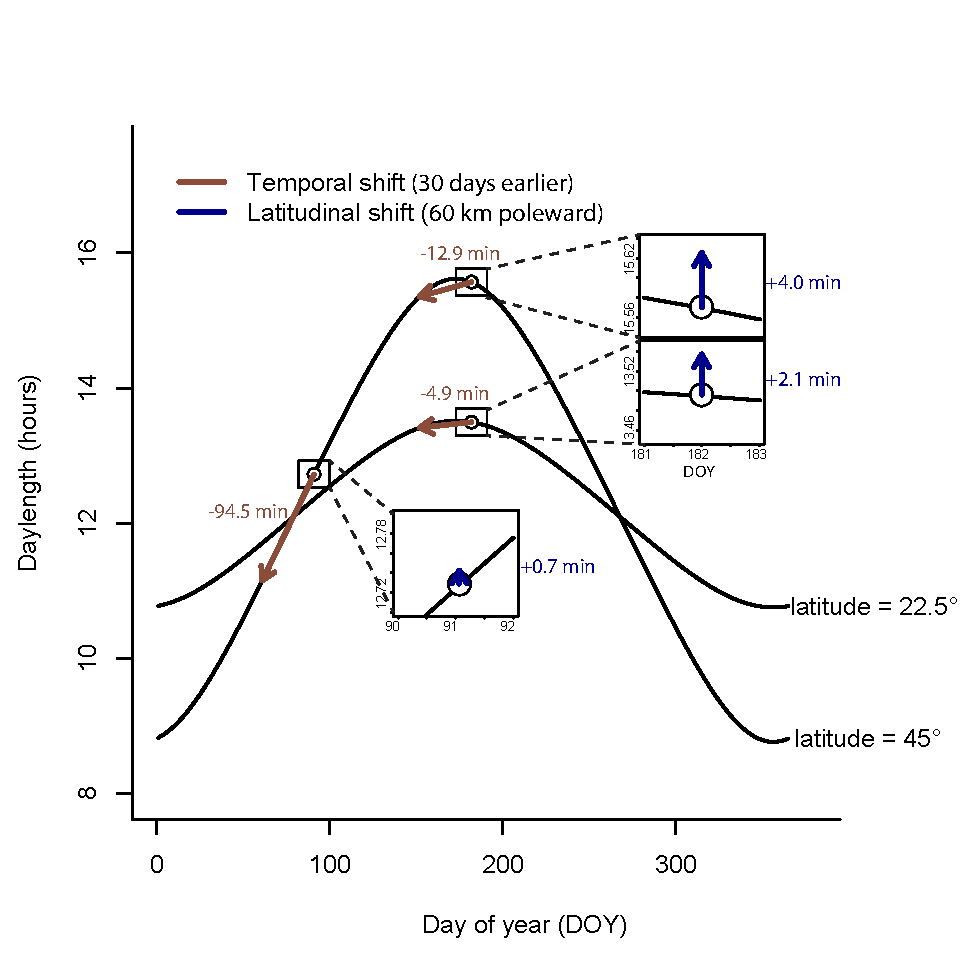
\includegraphics[scale=.6]{..//..//..//analyses/photoperiod/figures/photo_spacetime_v2a.pdf} %
\caption{\textbf{
\\\\Figure 1. Temporal (i.e., phenological) shifts in activity yield larger changes in experienced photoperiod compared to spatial (i.e., latitudinal) shifts} on the same day of year, due to patterns in photoperiod variation with latitude and by day of year. Here, we show this variation at two latitudes (22.5\degree, 45\degree), using hypothetical spatial and temporal shifts. These shifts are based on observed rates with recent global warming: 6-17 kilometers per decade, or approximately 0.5-1.5 degrees in 100 years, for spatial shifts (\emph{11,12}), and 2-3 days per decade, or 30 days in 100 years, for temporal shifts (\emph{12,13}). They highlight the greater magnitude in daylength changes in the early spring, close to the vernal equinox (e.g., day of year 91), versus close to the summer solstice (e.g., day of year 182).}
 \label{fig:spacetime}%
 \end{figure}
 
\begin{figure}
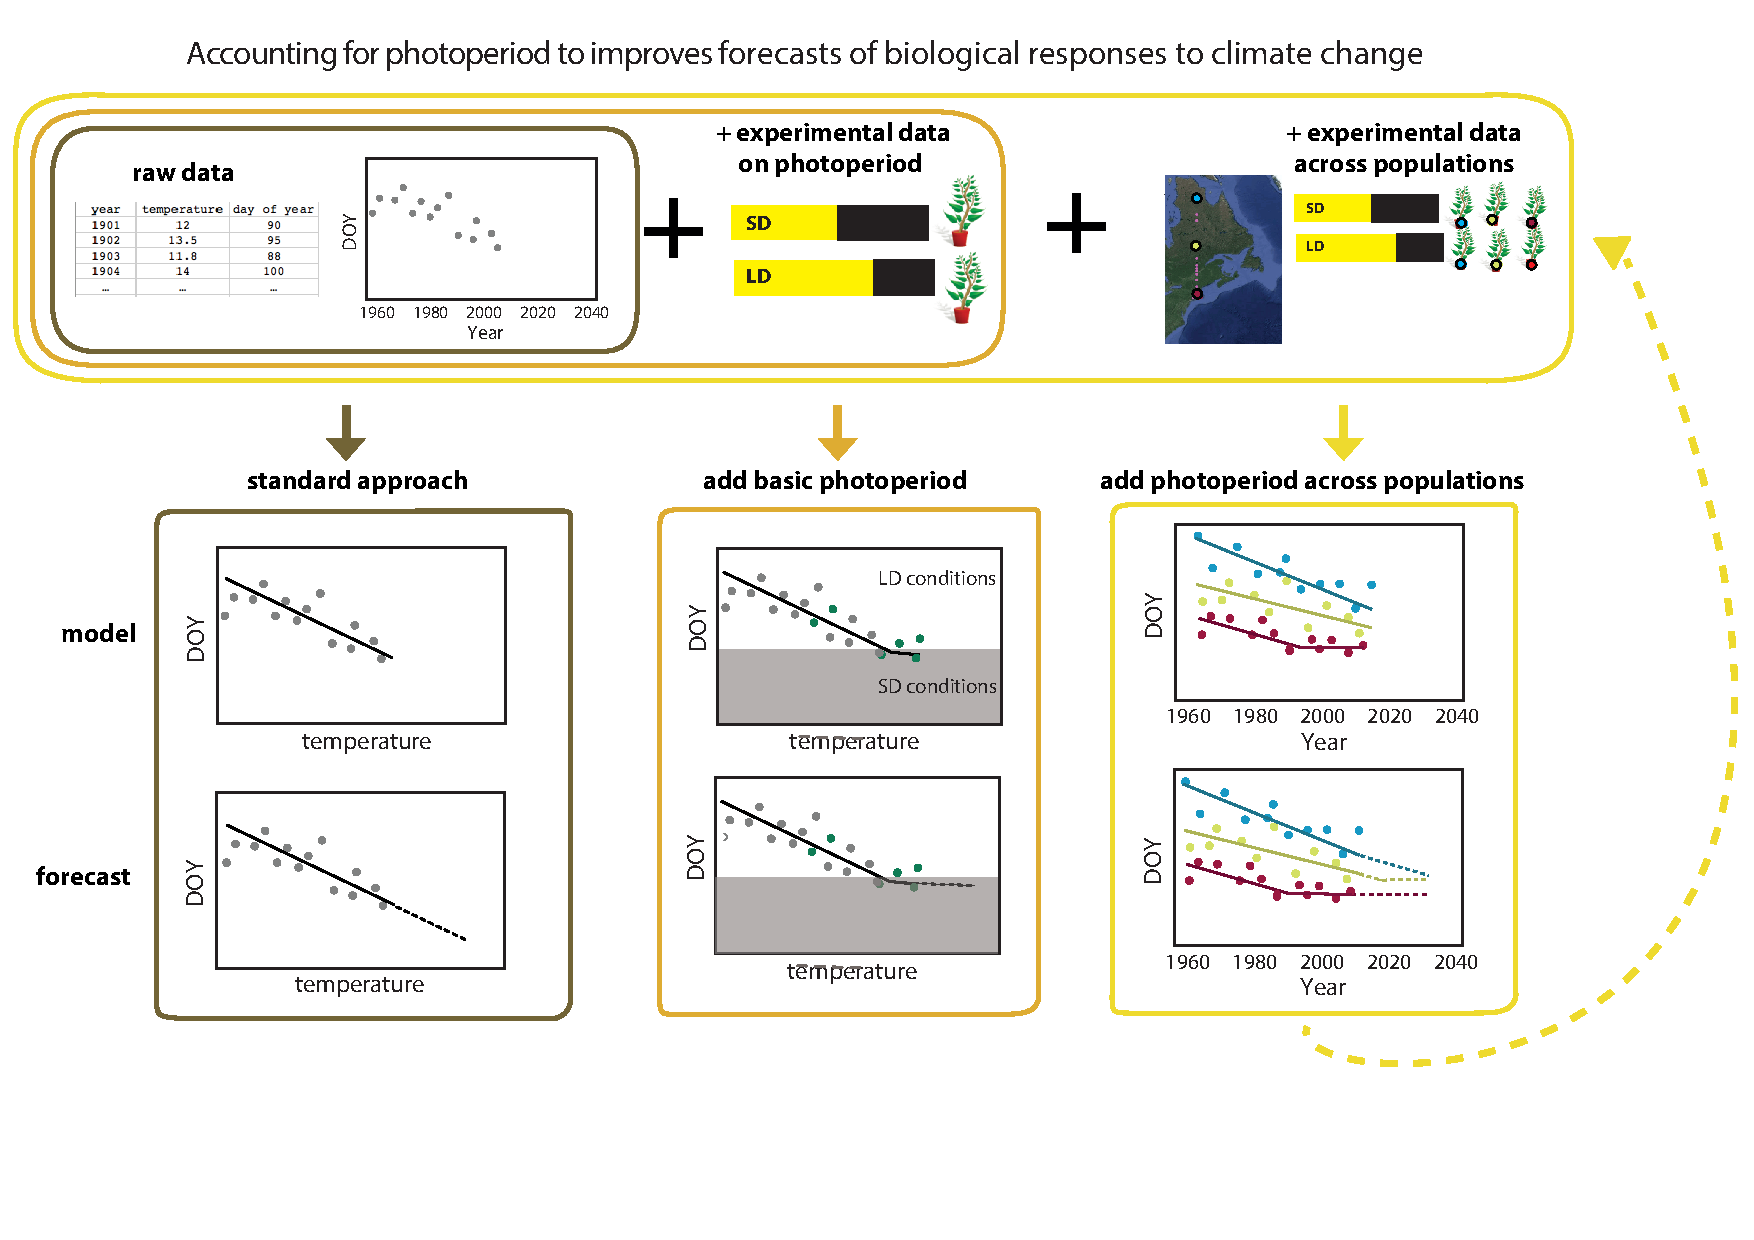
\includegraphics[scale=.55]{..//..//..//analyses/photoperiod/figures/photocondiag6.pdf} 
\caption{\textbf{Figure 2. Conceptual diagram of how to include photoperiod in forecasting biological responses to climate change}. Current approaches for forecasting spring phenology with climate change frequently rely on linear relationships between historical temperature data and observed dates of spring phenology (left panels). Adding responses to photoperiod, which commonly operate as threshold responses to short days (SD) versus long days (LD), will alter these forecasts (center panel) in ways that differ across species with divergent threshold photoperiods. (Threshold photoperiod is the length of day that causes an organism to switch from a short-- to a long--day response, or vice verse). Other factors that interact with photoperiod, such as population-level variation in photoperiod responses, can be incorporated into forecasts to further improve their accuracy (right panel).}
\label{fig:condiag}
\end{figure}
 
 \noindent \emph{References in cover letter and proposed abstract/figures}

\begin{enumerate}
\item Wolkovich, E.M.,  et al. 2019. Observed Spring Phenology Responses in Experimental Environments (OSPREE). Knowledge Network for Biocomplexity. urn:uuid:b2ab2746-b830-4
\item Saikkonen, K., et al. 2012. Climate change-driven species' range shifts filtered by photoperiodism. \emph{Nature Climate Change}, 2:239.
\item Way DA, Montgomery RA. 2015. Photoperiod constraints on tree phenology, performance and migration in a warming world. \emph{Plant, Cell \& Environment}, 38:1725-36.
\item Chamberlain, C.J., et al. 2019. Rethinking false spring risk.  \emph{Global Change Biology}.
\item Richardson, A.D., et al. 2018. Ecosystem warming extends vegetation activity but heightens vulnerability to cold temperatures. \emph{Nature}, 560: 368.
\item Fu, Y.H., et al. 2019. Daylength helps temperate deciduous trees to leaf-out at the optimal time. \emph{Global change biology}.
\item Fu, Y. S. H. et al. 2015. Declining global warming effects on the phenology of spring leaf unfolding. \emph{Nature} 526, 104-107.
\item Flynn D.F. \& Wolkovich EM. 2018. Temperature and photoperiod drive spring phenology across all species in a temperate forest community. \emph{New Phytologist}, 219:1353-62.
\item Wolkovich, E.M.,  et al. 2011. Warming experiments underpredict plant phenological responses to climate change. \emph{Nature} 485: 494.
\item Ettinger, A. K., et al. 2019. How do climate change experiments alter plot-scale climate?. \emph{Ecology letters}, 22: 748-763.
\item Parmesan and Yohe. 2003. A globally coherent fingerprint of climate change impacts across natural systems. \emph{Nature}, 21: 37-42.
\item Parmesan, C. 2006. Ecological and evolutionary responses to recent climate change. \emph{Annu. Rev. Ecol. Evol. Syst}, 37:637-69
\item Chen, C. et al 2011. Rapid range shifts of species associated with high levels of climate warming. \emph{Science}, 333: 1024-1026.
 \end{enumerate}
\end{footnotesize}

\end{letter}
\end{document}
